\documentclass[11pt]{article}
\usepackage[margin=0.75in]{geometry}
\usepackage{amsmath}
\usepackage{enumitem}
\usepackage{tikz,soul}

\usepackage{multicol}

\newcommand{\ds}{\displaystyle}

\begin{document}
\newcounter{enumCount}
\pagestyle{empty}
\subsection*{Math 105 - Homework 5 \hfill Name: \underline{\hspace*{2in}}}


\noindent 
\textit{In each problem below, find an equation for the line that fits the description.}
\begin{multicols}{2}
\begin{enumerate}
\setcounter{enumi}{\theenumCount}
\item Passes through $(1,-2)$ and $(3,4)$.
\item Passes through $(-4,5)$ and $(8,2)$ 
\setcounter{enumCount}{\theenumi}
\end{enumerate}
\end{multicols}
\vfill




\begin{multicols}{2}
\begin{enumerate}
\setcounter{enumi}{\theenumCount}
\item Has a slope of 5 and crosses the $x$-axis at $x=3$.
\item Passes through $(3,4)$ with slope of $-6$.
\setcounter{enumCount}{\theenumi}
\end{enumerate}
\end{multicols}
\vfill


\begin{enumerate}
\setcounter{enumi}{\theenumCount}
\item Find the slope and $y$-intercept of the line $4x + 6y = 24$.
\vfill


\item Suppose that there are 4 inches of snow already on the ground when a new snow storm arrives.  During the storm, snow falls at a rate of 2/3 of an inch per hour.  Find a formula for the depth of the snow on the ground ($y$) as a function of the number of hours ($x$) that have passed since the storm started. 
\vfill

\item At this rate, how long would it be until the snow is 1 foot (12 inches) deep?  
\vfill


\newpage

\item  Suppose that the cost for a business to manufacture $x$ widgets is $C(x)$ dollars.  Explain in words what the following equation means:
$$C(5{,}000) = 6{,}000.$$
\vfill
\setcounter{enumCount}{\theenumi}
\end{enumerate}



\noindent
\textit{Suppose that $f(x) = \dfrac{1}{x+2}$ and $g(x) = 4x+3$.}
\begin{multicols}{2}
\begin{enumerate}
\setcounter{enumi}{\theenumCount}
\item Calculate $f(g(0))$.
\item Calculate $g(f(0))$.
\setcounter{enumCount}{\theenumi}
\end{enumerate}
\end{multicols}
\vfill

\noindent
\textit{The following graphs show two different functions $f(x)$ and $g(x)$.}

\begin{center}
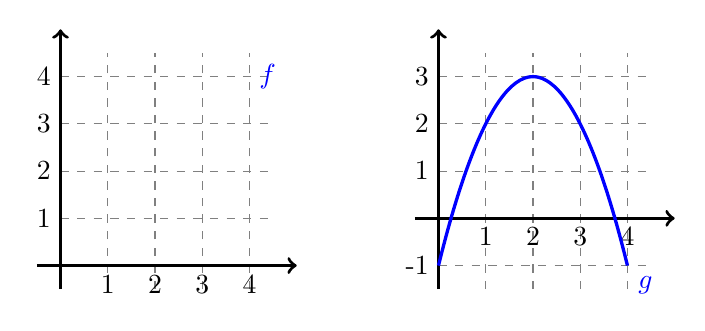
\begin{tikzpicture}[scale=0.6]
\draw[dashed, gray] (0,-0.5) grid (4.5,4.5);
\draw[very thick,->] (-0.5,0) -- (5,0);
\draw[very thick,->] (0,-0.5) -- (0,5);
\foreach \i in {1,...,4} {
  \draw (\i,0) node[below] {\i};
  \draw (0,\i) node[left] {\i};
}
\draw[very thick,color=blue] plot[domain=-0.5:4.1,samples=100] function {4/(5-x)};
\draw[color=blue] (4,4) node[right] {$f$};
\begin{scope}[xshift=8cm, yshift=1cm]
\draw[dashed, gray] (0,-1.5) grid (4.5,3.5);
\draw[very thick,->] (-0.5,0) -- (5,0);
\draw[very thick,->] (0,-1.5) -- (0,4);
\foreach \i in {1,...,4} {
  \draw (\i,0) node[below] {\i};
}
\foreach \i in {-1,1,2,3} {
  \draw (0,\i) node[left] {\i};
}
\draw[very thick, blue] (0,-1) parabola bend (2,3) (4,-1) node[below right] {$g$};
\end{scope}
\end{tikzpicture}
\end{center}
\textit{Use the graphs to evaluate the following.}
\begin{multicols}{3}
\begin{enumerate}
\setcounter{enumi}{\theenumCount}
\item $f(g(2))$
\item $g(f(1))$ 
\item $g(f(4))$ 
\setcounter{enumCount}{\theenumi}
\end{enumerate}
\end{multicols}
\vfill


\textit{Simplify the following products by expanding.  As always, show your work.} % No calculators.} 

\begin{multicols}{2}
\begin{enumerate}
\item $y = \dfrac{1}{x-3}$ \\
\begin{center}
\begin{tikzpicture}
\draw[thick,->] (-2,0) -- (2,0);
\draw[thick,->] (0,-2) -- (0,2);
\end{tikzpicture}
\end{center}

\item $y = \sqrt{x} + 3$ \\
\begin{center}
\begin{tikzpicture}
\draw[thick,->] (-2,0) -- (2,0);
\draw[thick,->] (0,-2) -- (0,2);
\end{tikzpicture}
\end{center}
\setcounter{enumCount}{\theenumi}
\end{enumerate}
\end{multicols}


\begin{multicols}{2}
\begin{enumerate}
\setcounter{enumi}{\theenumCount}
\item $y = \dfrac{x^2}{4}$ \\
\begin{center}
\begin{tikzpicture}
\draw[thick,->] (-2,0) -- (2,0);
\draw[thick,->] (0,-2) -- (0,2);
\end{tikzpicture}
\end{center}

\item $y = -(x+1)^2$ \\
\begin{center}
\begin{tikzpicture}
\draw[thick,->] (-2,0) -- (2,0);
\draw[thick,->] (0,-2) -- (0,2);
\end{tikzpicture}
\end{center}
\setcounter{enumCount}{\theenumi}
\end{enumerate}
\end{multicols}

\noindent
\textit{Solve the following equations.} 
\begin{multicols}{2}
\begin{enumerate}
\setcounter{enumi}{\theenumCount}
\item $\dfrac{1}{x-3} = 2$ 

\item $\sqrt{x} + 3 = 12$ 
\setcounter{enumCount}{\theenumi}
\end{enumerate}
\end{multicols}
\vfill

\begin{multicols}{2}
\begin{enumerate}
\setcounter{enumi}{\theenumCount}
\item $\dfrac{x^2}{4} = 25$ 

\item $-(x+1)^2 = -9$ 
\setcounter{enumCount}{\theenumi}
\end{enumerate}
\end{multicols}
\vfill


\begin{multicols}{2}
\begin{enumerate}
\setcounter{enumi}{\theenumCount}
\item $\dfrac{5}{x} = \dfrac{2}{3}$ 

\item $\dfrac{x}{4-x} = 3$ 
\setcounter{enumCount}{\theenumi}
\end{enumerate}
\end{multicols}
\vfill

\end{document}
